Un mono trepa de manera vertical. Su movimiento se muestra en la siguiente gráfica (Fig. \ref{fig:dist_tiempo_03}) de la posición vertical,
$y$, en funci\'on del tiempo, $t$. \par

{\InsertBoxR{0}{
        \parbox[t]{0.5\linewidth}{
            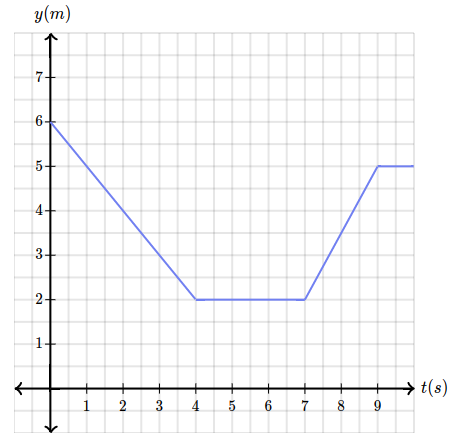
\includegraphics[width=\linewidth]{Images/dist_tiempo_03}
            \label{fig:dist_tiempo_03}
            \captionof{figure}{La gráfica representa el movimiento del mono.}%
        }
    }}
\hspace{0.5cm}
\begin{minipage}[t]{0.4\linewidth}
    \begin{parts}
        % \begin{minipage}[t]{0.45\linewidth}
        % \include*{Questions/Parts/question007a}
        % \include*{Questions/Parts/question007d}
        %\end{minipage}%

        \include*{Questions/Parts/question007c}
        \include*{Questions/Parts/question007b}
        \include*{Questions/Parts/question007e}
        %\include*{Questions/Parts/question007f}
        %\include*{Questions/Parts/question007g}
        \include*{Questions/Parts/question007h}
    \end{parts}
\end{minipage}
